% - frame -----------------------------------------------------------------
\begin{frame}
   \frametitle{Motivace}
   \begin{columns}[t, onlytextwidth]
      \begin{column}[T]{0.5\textwidth}
         \begin{itemize}
            \item \textbf{Mobot} - ovladač mobilních telefonů
		\begin{itemize}
			\item Manipulátor a kamera pro náhradu lidské interakce s telefonem
		\end{itemize}
		\item Pro konfiguraci nových telefonů
		\item Spolupráce se Škoda Auto
		\item Umí detekovat telefon na pracovní ploše
         \end{itemize}
      \end{column}
      \begin{column}[T]{0.49\textwidth}
         \centering
         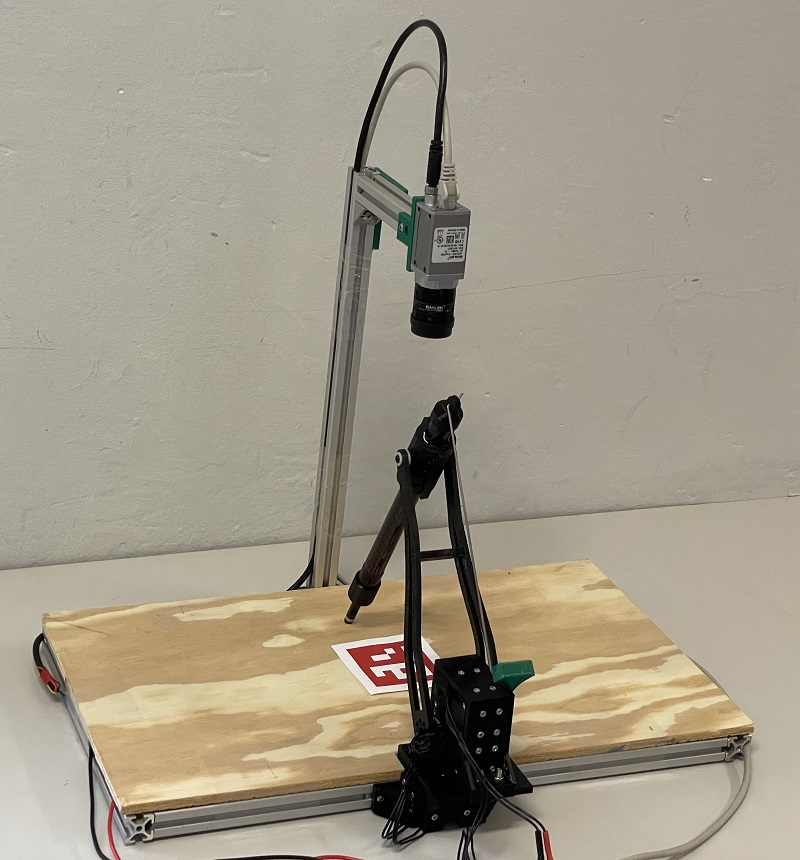
\includegraphics[width=0.8\linewidth]{mobot.JPG}
      \end{column}
   \end{columns}
\end{frame}

% - frame -----------------------------------------------------------------
\begin{frame}
   \frametitle{Příprava datasetu}
   \begin{columns}[t, onlytextwidth]
      \begin{column}[T]{0.5\textwidth}
         \begin{itemize}
            \item Nasbírání 100 fotek \emph{různých} telefonů
            \item Pro labelování použito \textbf{labelme} - časově náročné :(
            \item Převedení do jiného formánu vhodného pro trénování architektury \textbf{YOLOv5} za pomoci \textbf{RoboFlow}
            \item Rozšíření datasetu pomocí \textbf{augmentací}
         \end{itemize}
      \end{column}
      \begin{column}[T]{0.49\textwidth}
         \centering
         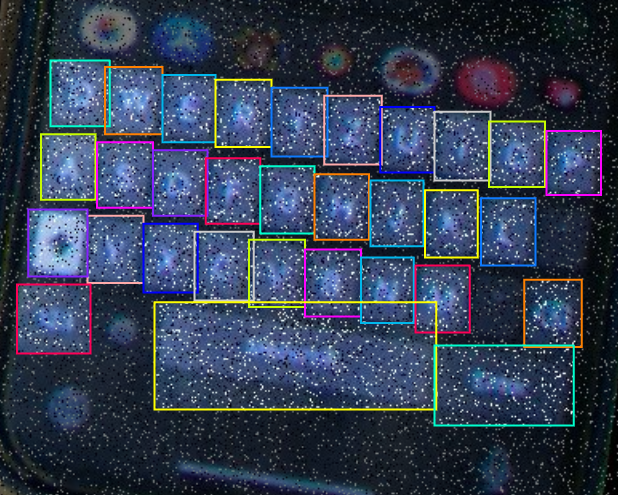
\includegraphics[width=0.8\linewidth]{labeling_demonstration.png}
      \end{column}
   \end{columns}
\end{frame}

% - frame -----------------------------------------------------------------
\begin{frame}
   \frametitle{Architektura a trénování}
   \begin{columns}[t, onlytextwidth]
      \begin{column}[T]{0.44\textwidth}
         \begin{itemize}
            \item Použita základní architektura \textbf{YOLOv5}, která umožnila detekovat více objektů najednou
            \parbox{\textwidth}{\tiny {\color{ctu4blue}Nelson J.}: \url{https://www.youtube.com/watch?v=MdF6x6ZmLAY}.}
            \item Konfigurace \textbf{s} (small) vhodná pro rychlé trénování
            \item Trénování proběhlo v \textbf{Google Colab}
         \end{itemize}
      \end{column}
      \begin{column}[T]{0.55\textwidth}
         \centering
         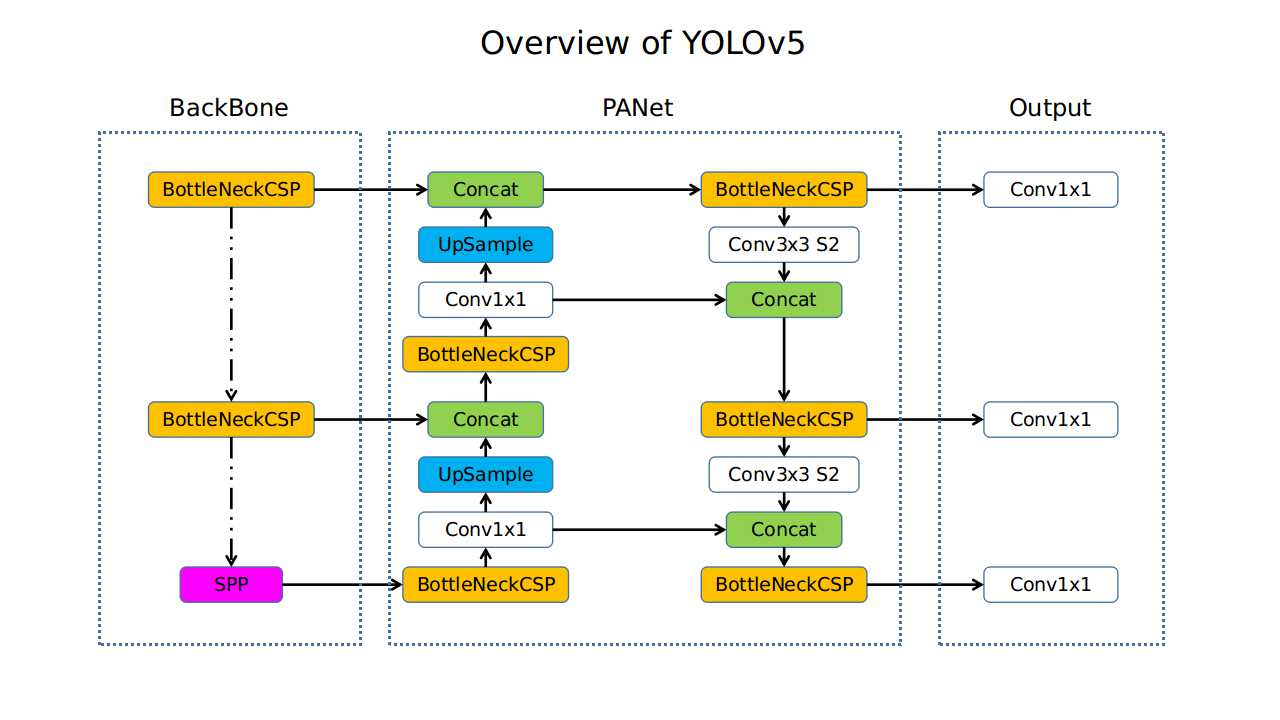
\includegraphics[width=\linewidth]{yolov5_arch.jpg}
      \end{column}
   \end{columns}
\end{frame}

% - frame -----------------------------------------------------------------
\begin{frame}
   \frametitle{Průběh trénování}
   \begin{columns}[t, onlytextwidth]
      \begin{column}[T]{0.44\textwidth}
      \begin{itemize}
         \item Nejlepších parametrů klasifikace bylo dosaženo s velmi \textbf{augmentovaným} datasetem a \textbf{1100} epochami
      \end{itemize}
         \centering
         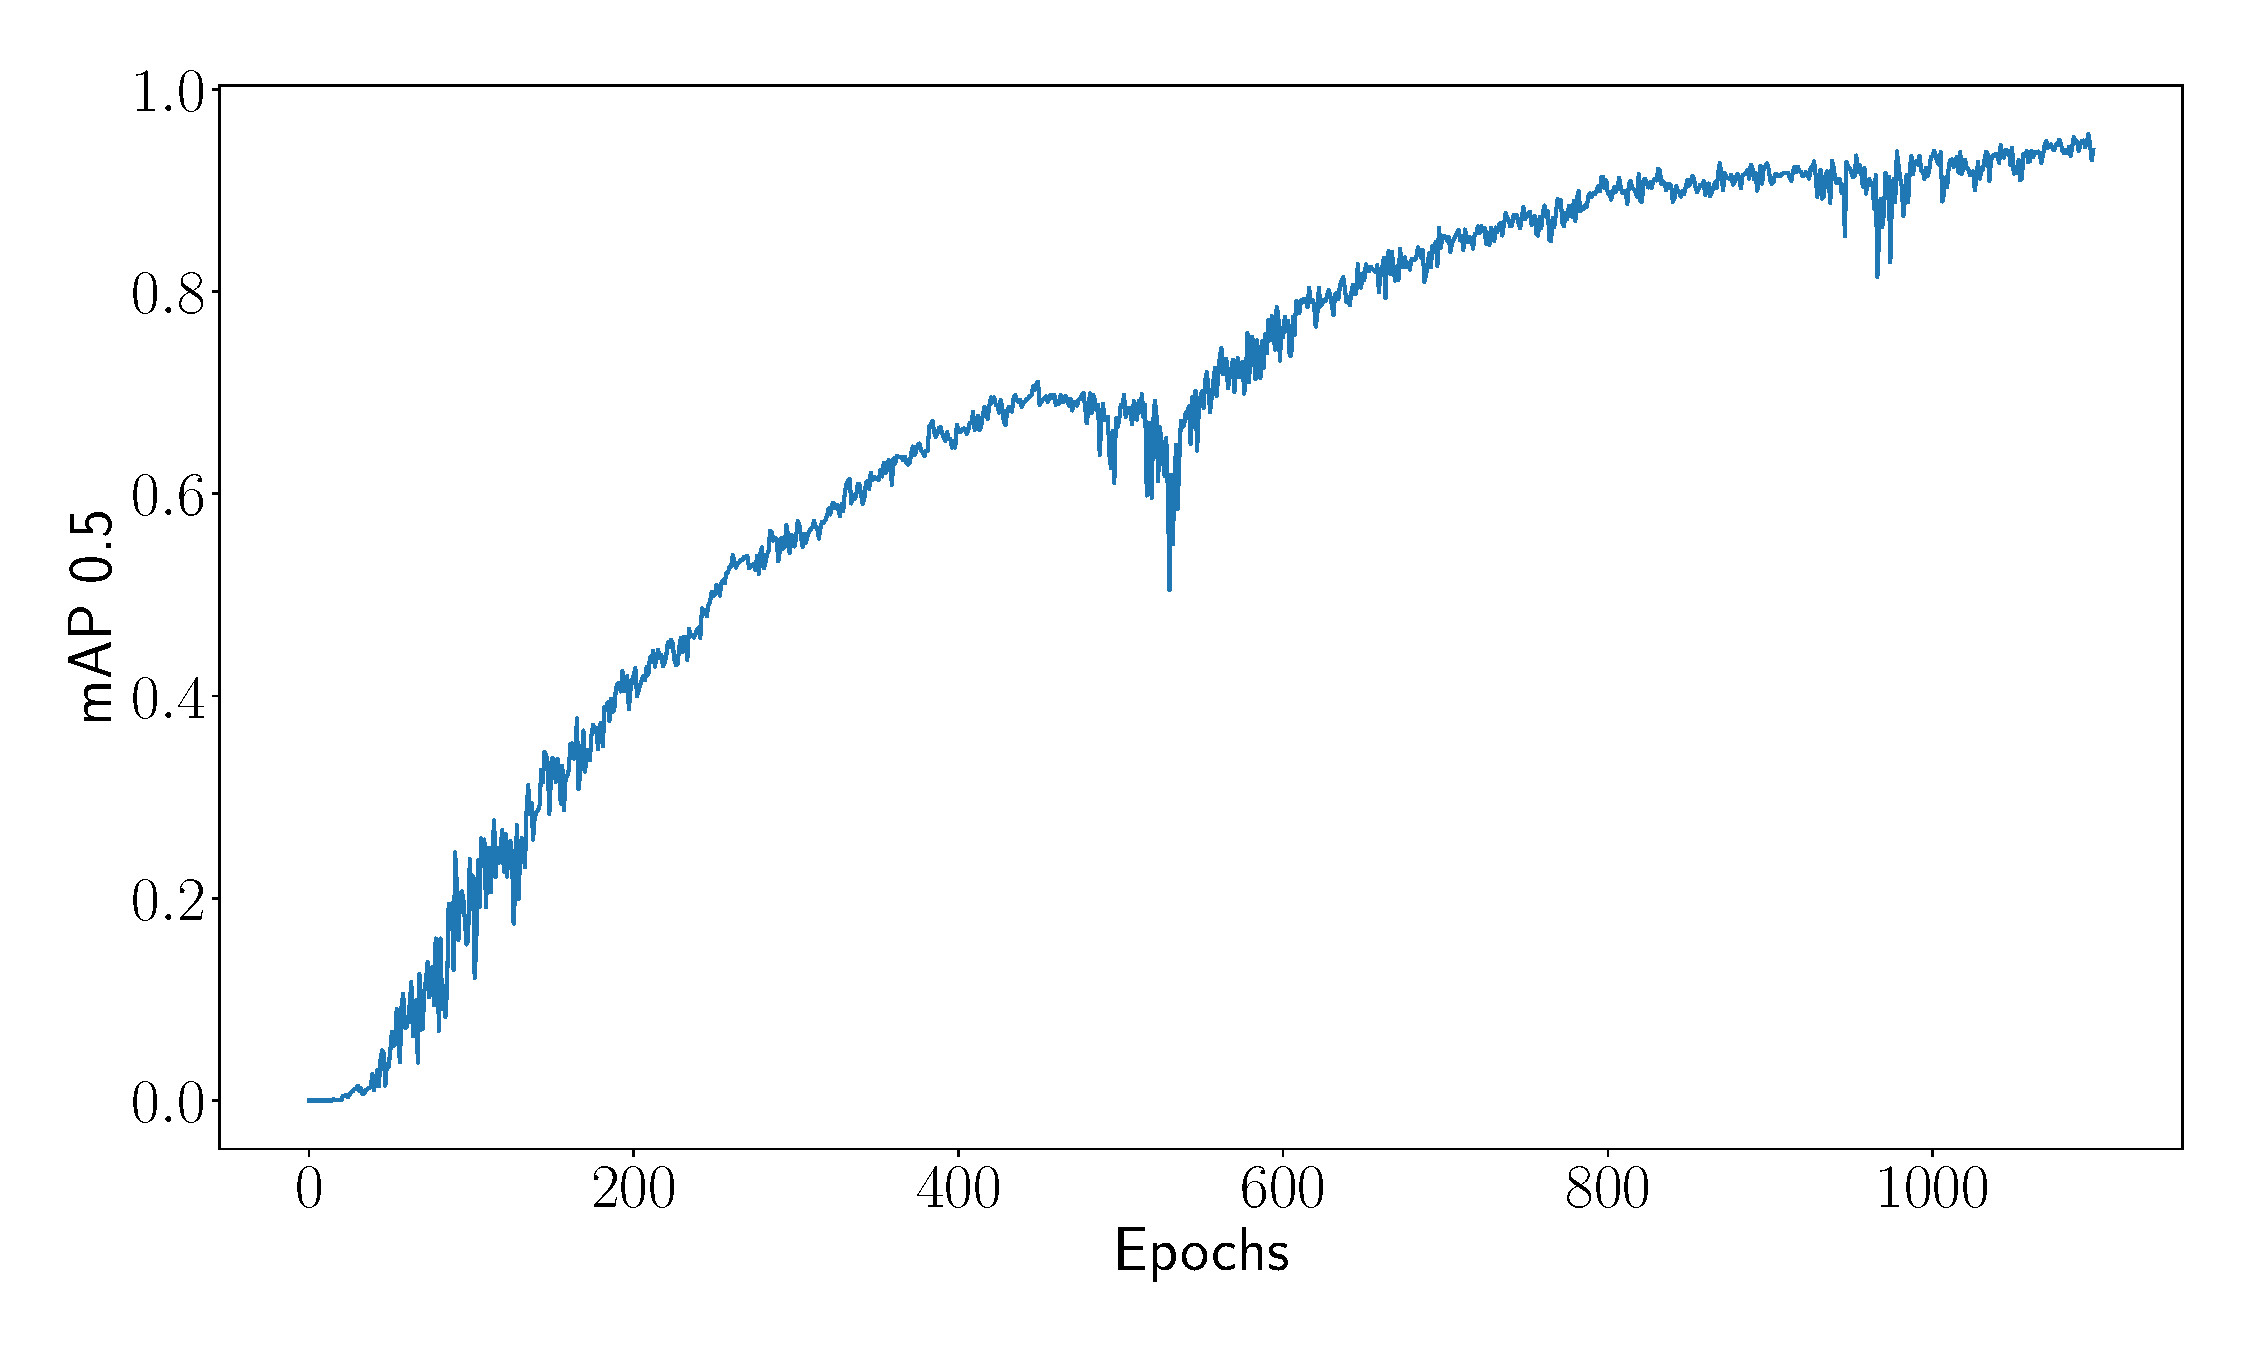
\includegraphics[width=\linewidth]{map.pdf}
      \end{column}
      \begin{column}[T]{0.55\textwidth}
         \centering
         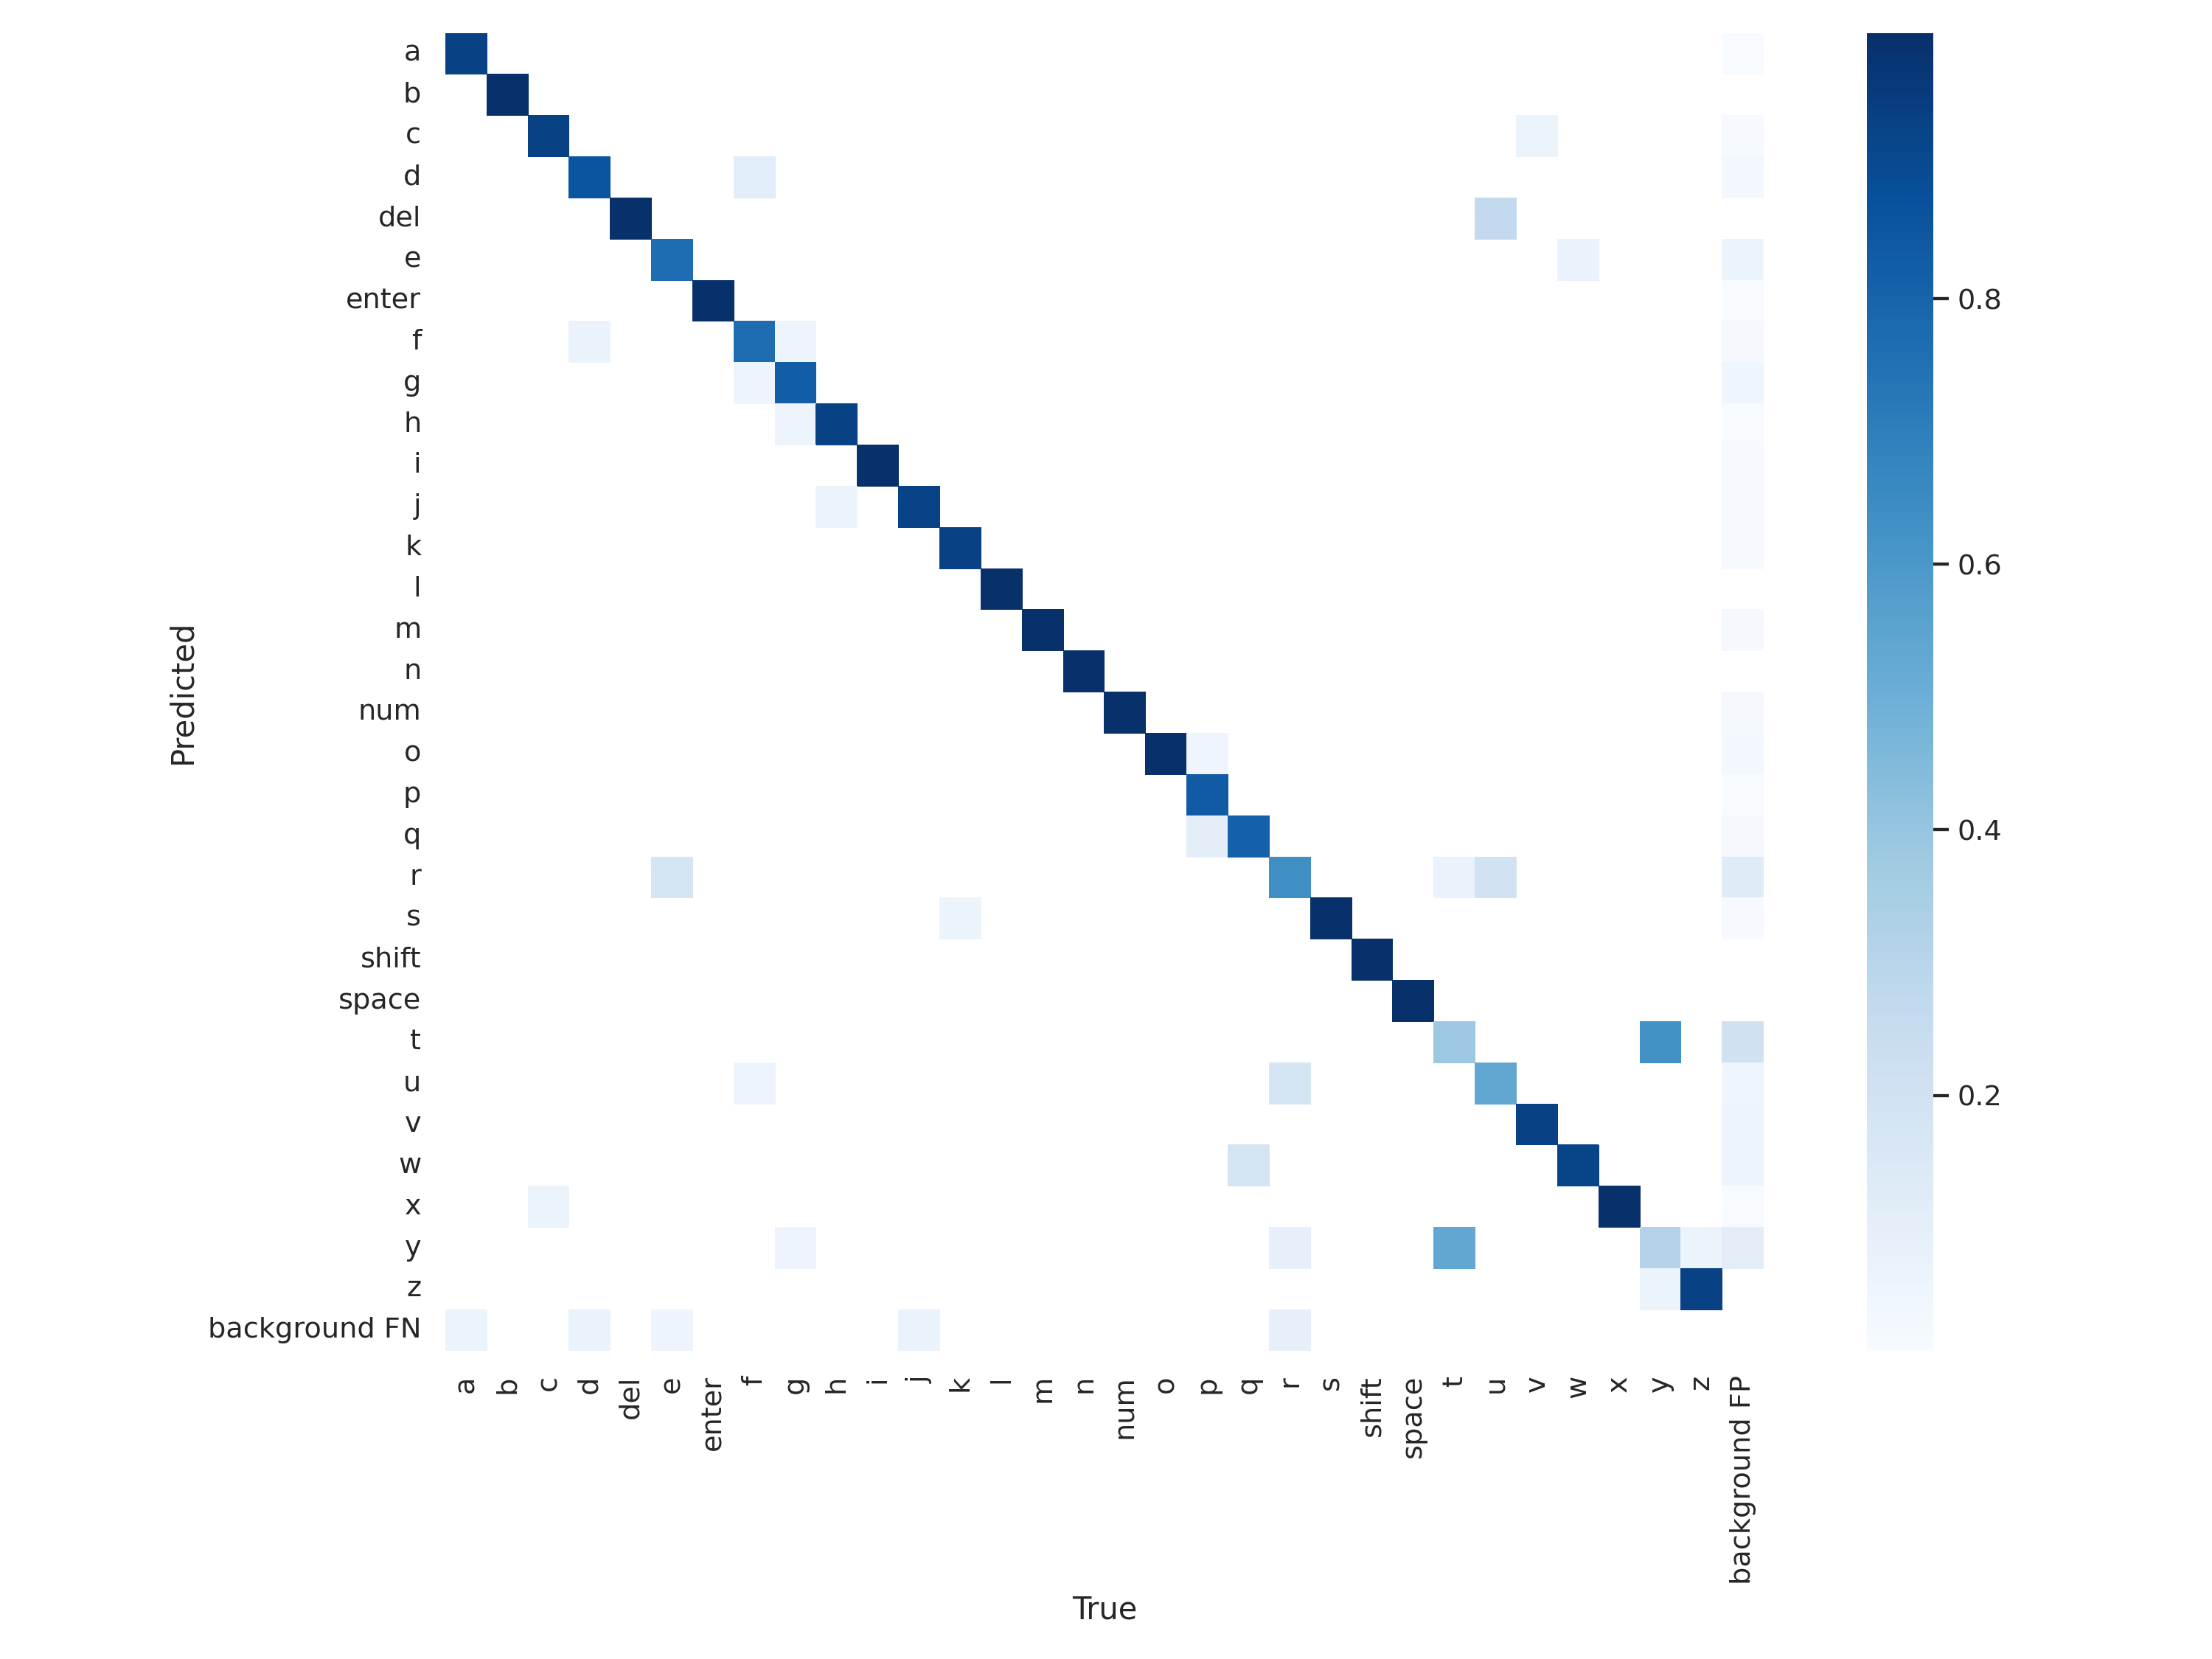
\includegraphics[width=\linewidth]{confusion_matrix_1100.png}
      \end{column}
   \end{columns}
\end{frame}

% - frame -----------------------------------------------------------------
\begin{frame}
   \frametitle{Detekce}
   \begin{columns}[t, onlytextwidth]
      \begin{column}[T]{0.5\textwidth}
         \begin{figure}[h]
         		\centering
         		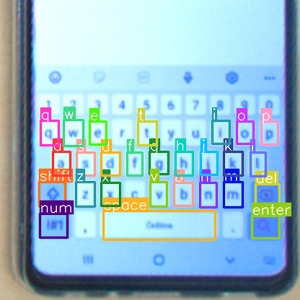
\includegraphics[]{detect40.png}
			\caption{Detection of small letters}
		\end{figure}
      \end{column}
      \begin{column}[T]{0.50\textwidth}
		\begin{figure}[h]
         		\centering
         		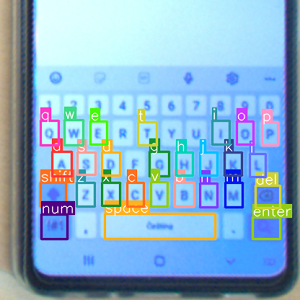
\includegraphics[]{detect40Big.png}
			\caption{Detection of big letters}
		\end{figure}
      \end{column}
   \end{columns}
\end{frame}

% - frame -----------------------------------------------------------------
\begin{frame}
   \frametitle{Postprocesing}
   \begin{columns}[t, onlytextwidth]
      \begin{column}[T]{0.5\textwidth}
         \begin{figure}[h]
         		\centering
         		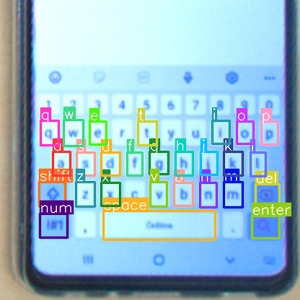
\includegraphics[]{detect40.png}
			\caption{Detekované klávesy}
		\end{figure}
      \end{column}
      \begin{column}[T]{0.50\textwidth}
		\begin{figure}[h]
         		\centering
         		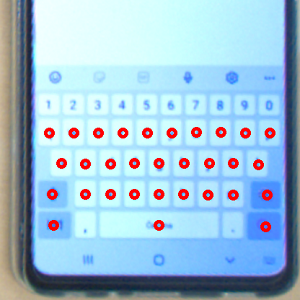
\includegraphics[]{completed.png}
			\caption{Celá klávesnice s body pro robota}
		\end{figure}
      \end{column}
   \end{columns}
\end{frame}

% - frame -----------------------------------------------------------------
\begin{frame}
   \frametitle{Postprocesing 2}
   \begin{columns}[t, onlytextwidth]
      \begin{column}[T]{0.5\textwidth}
         \begin{figure}[h]
         		\centering
         		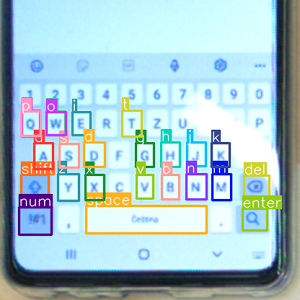
\includegraphics[]{postErrSource.png}
			\caption{Špatně detekované klávesy}
		\end{figure}
      \end{column}
      \begin{column}[T]{0.50\textwidth}
		\begin{figure}[h]
         		\centering
         		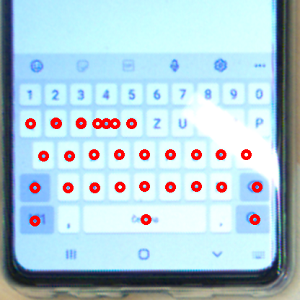
\includegraphics[]{postErr.png}
			\caption{Chybně doplněná klávesnice}
		\end{figure}
      \end{column}
   \end{columns}
\end{frame}

% - frame -----------------------------------------------------------------
\begin{frame}
   \frametitle{Postprocesing 3}
   \begin{columns}[t, onlytextwidth]
      \begin{column}[T]{0.5\textwidth}
         \begin{figure}[h]
         		\centering
         		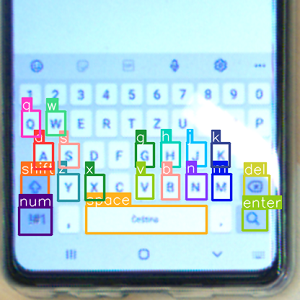
\includegraphics[]{detect60.png}
			\caption{Detekce se zvýšeným prahem důvěry na 60 \%}
		\end{figure}
      \end{column}
      \begin{column}[T]{0.50\textwidth}
		\begin{figure}[h]
         		\centering
         		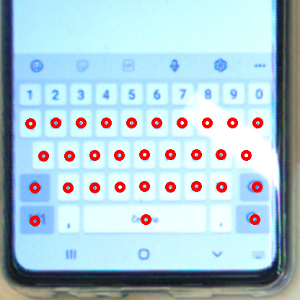
\includegraphics[]{completedGlare.png}
			\caption{Správně doplněná klávesnice}
		\end{figure}
      \end{column}
   \end{columns}
\end{frame}

% - frame -----------------------------------------------------------------
\begin{frame}
   \frametitle{Budoucí práce}
   \begin{columns}[t, onlytextwidth]
      \begin{column}[T]{0.5\textwidth}
         	\begin{itemize}
            \item Implementace do programu ovládání Mobota
			\item Možná vylepšení:
			\begin{itemize}
				\item Detekce více kláves - lepší trénovací dataset
				\item Detekce České klávesnice - to nyní nefunguje
			\end{itemize}
        \end{itemize}

      \end{column}
      \begin{column}[T]{0.49\textwidth}
         \centering
         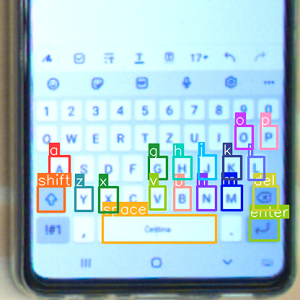
\includegraphics[width=0.8\linewidth]{detectCzErr.png}
      \end{column}
   \end{columns}
\end{frame}
